% !TeX spellcheck = en_US

\chapter{Concept Description}

	uFixit is a platform on which user can get manuals that help them repair things. It does not matter from which manufacturer it comes, it works with all products of either brand. There is only one minor constraint: The part has to be fixable.
	
	\begin{figure}[H]
		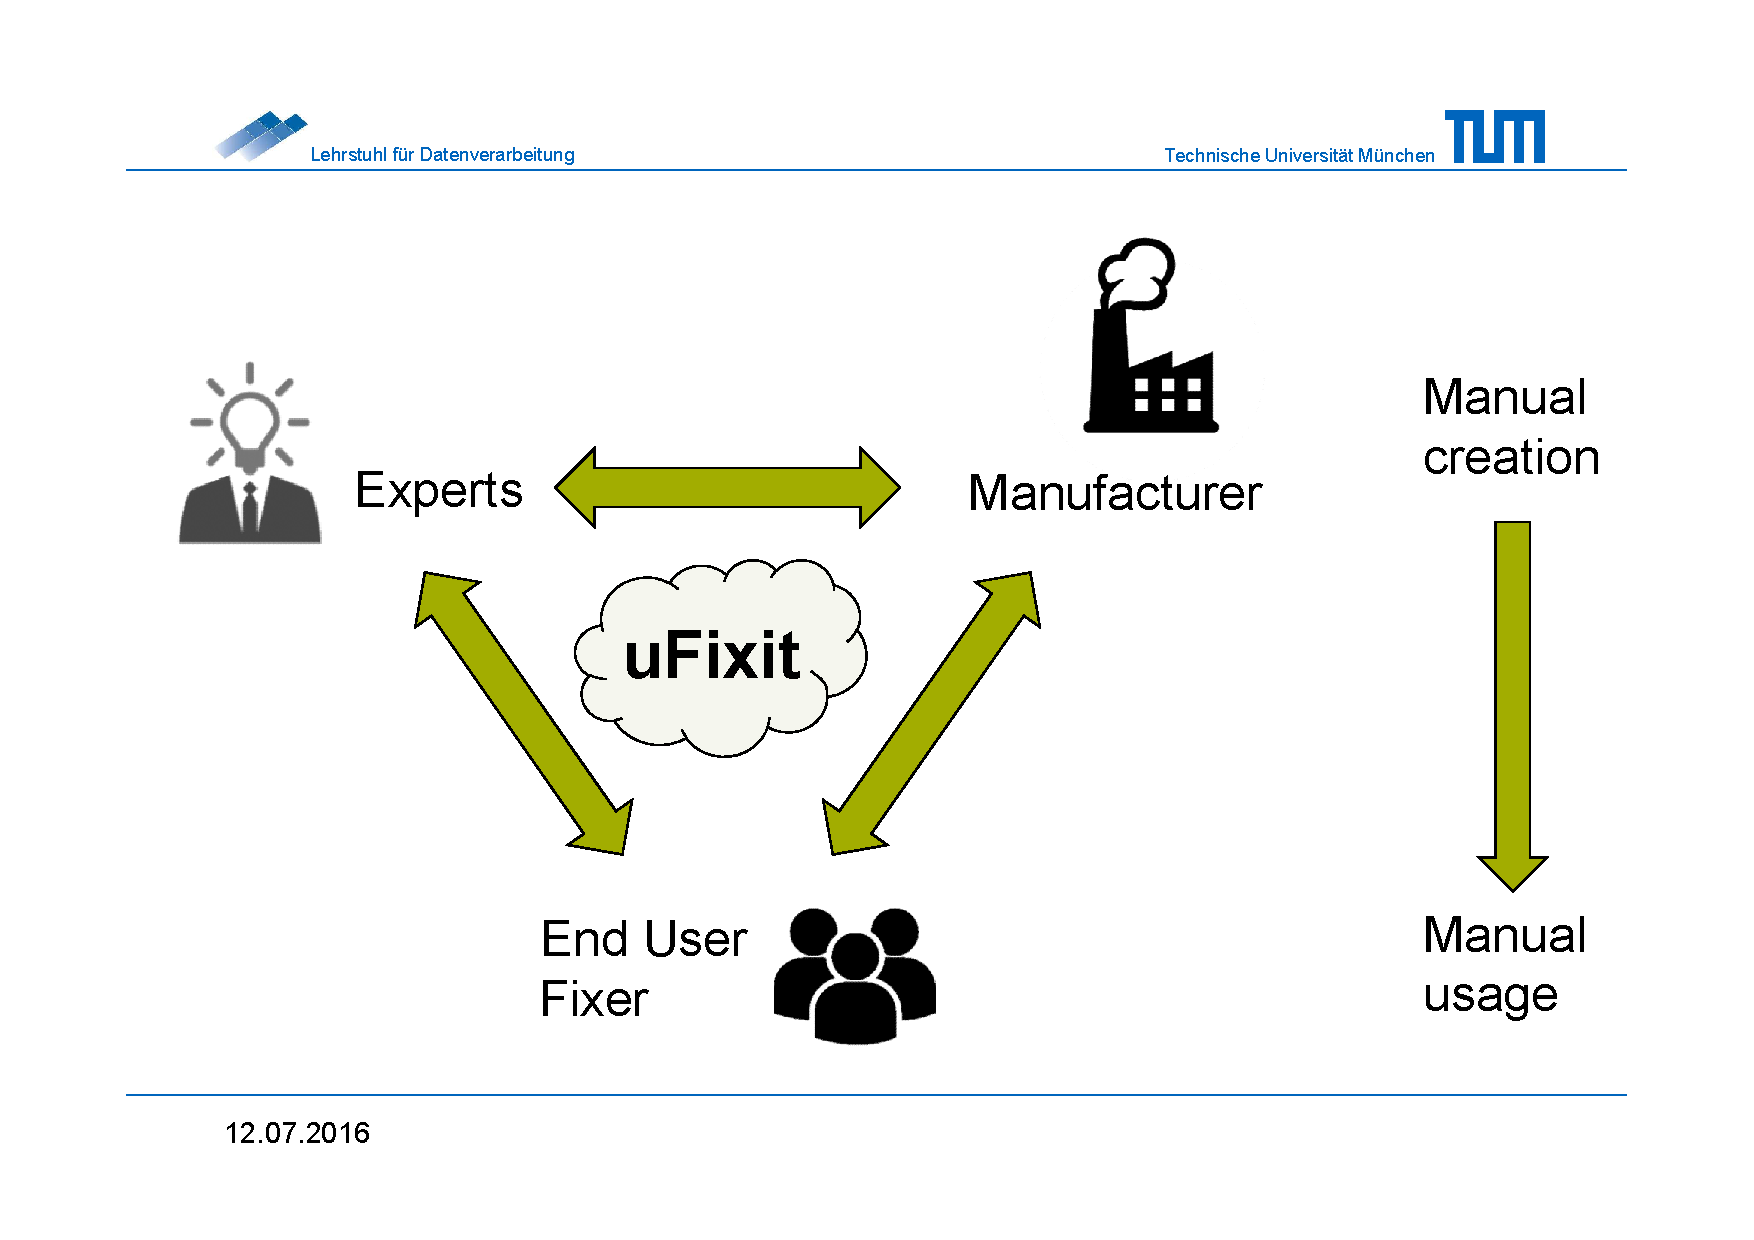
\includegraphics[width=\textwidth, trim=0cm 3cm 0cm 4cm, clip]{../images/involved-parties.pdf}
		\centering
		\caption{Parties involved in the uFixit environment}
		\label{fig:involved-parties}
	\end{figure}
	
	As one can see in \autoref{fig:involved-parties}, \textbf{Experts} and \textbf{Manufacturers} create the manuals, whereas \textbf{Fixers} use them on their own device. An Expert is a person that has the same equipment as the end user, but does create manuals. He will not have special training or software to do so. Manufacturers on the other side have detailed information and models of their products and therefore can develop high quality instruction steps with animations and extensive highlightings.
	
	After describing how the instructions inside a manual will look like, we discuss how uFixit helps experts as well as manufacturers in creating the best possible manuals for the end user.


	\section{Instructions format}
	
		Every manual will be separated into several individual steps. Each of these steps will ask the user to perform a specific task to fulfill. After that, the manual must transition to the next step. There are a few different possibilities:
		
		\begin{itemize}
			\itemsep0em
			\item The AR device constantly watches the fixer while performing the task. Due to sophisticated algorithms, the application can detect when it is finished and will automatically jump to the next one.
			\item Ideally the used device has a microphone built in. With that, the fixer simply can issue a voice command.
			\item Although it is more of a feature to jump to a specific step in the tutorial, forward and backward buttons will be provided on screen for easy access.
		\end{itemize}
		
		
		
		\begin{figure}[H]
			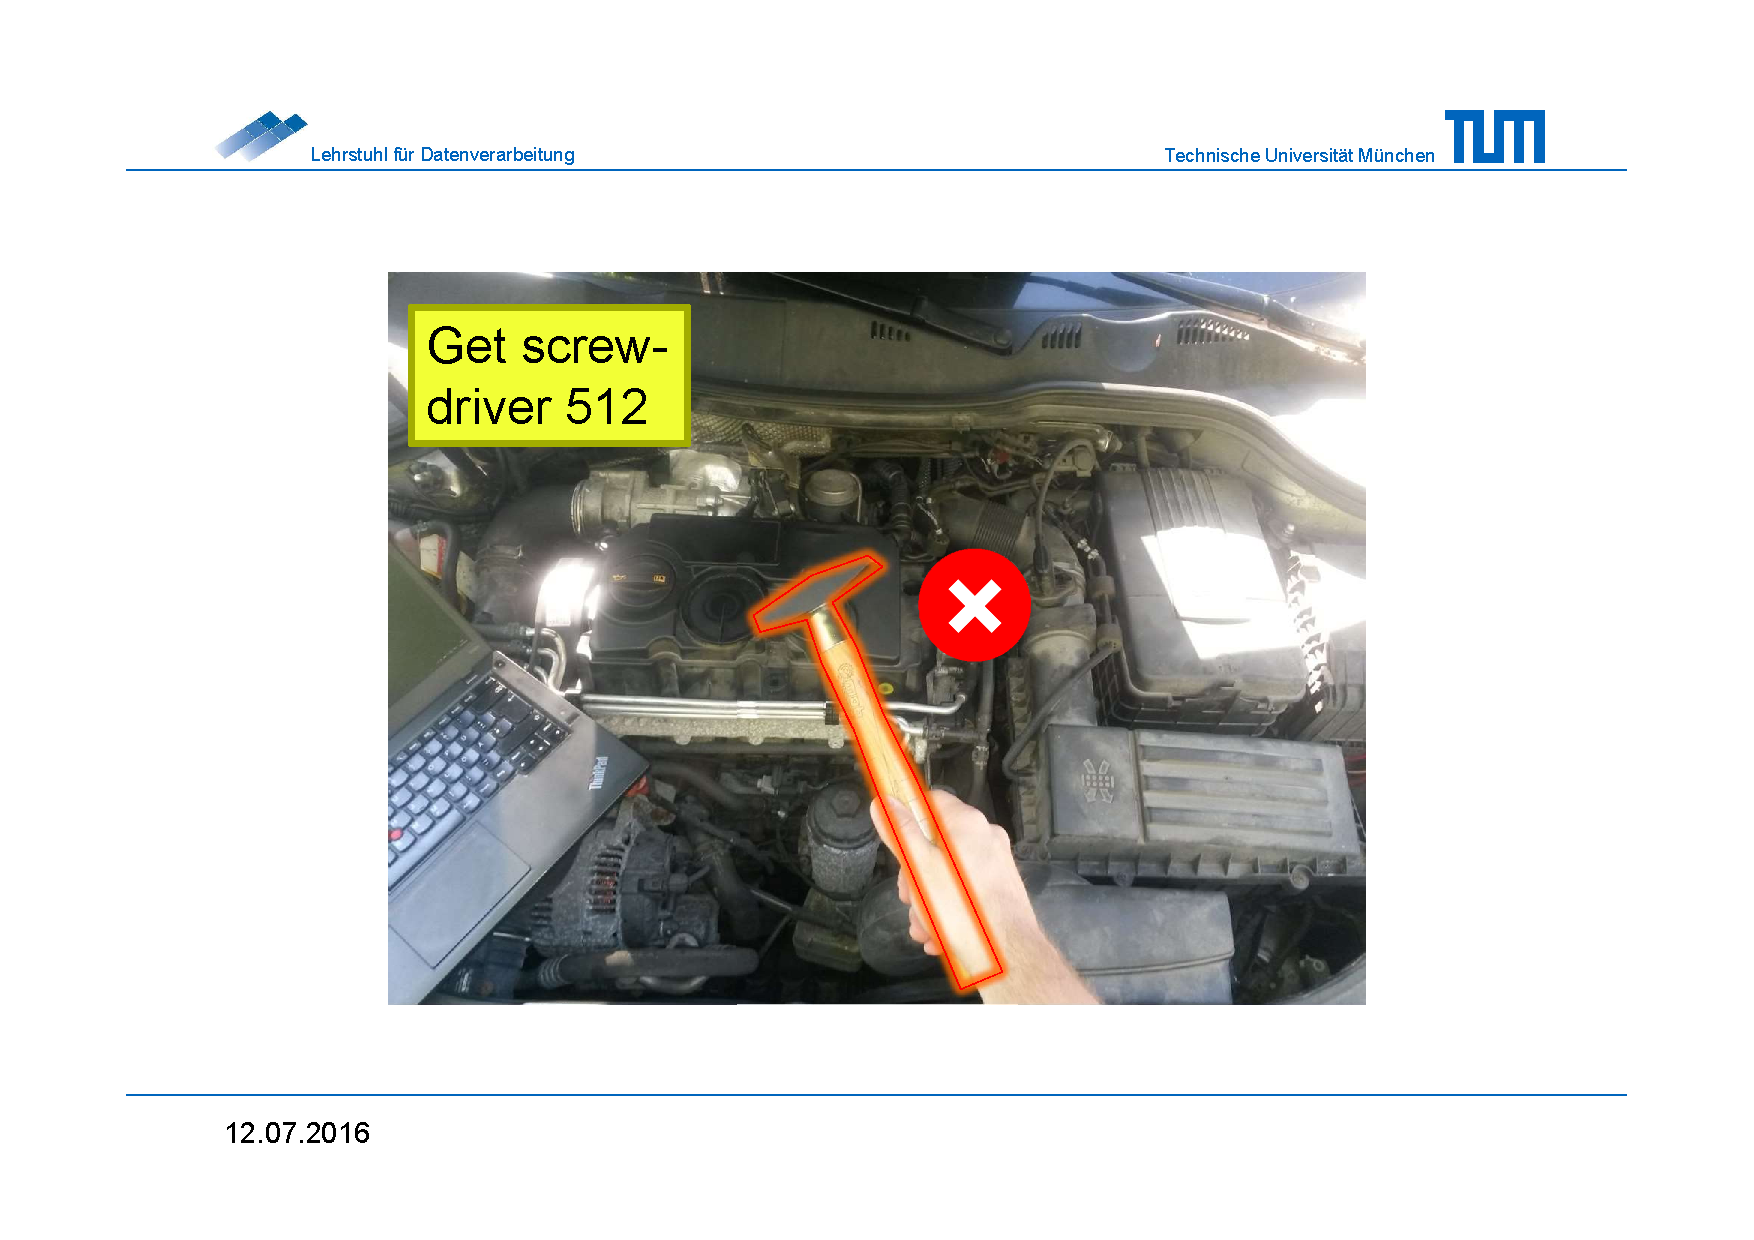
\includegraphics[width=\textwidth, trim=4cm 3cm 4cm 4cm, clip]{../images/instr-hammer.pdf}
			\centering
			\caption{Parties involved in the uFixit environment}
			\label{fig:instr-hammer}
		\end{figure}
		
		\begin{figure}[H]
			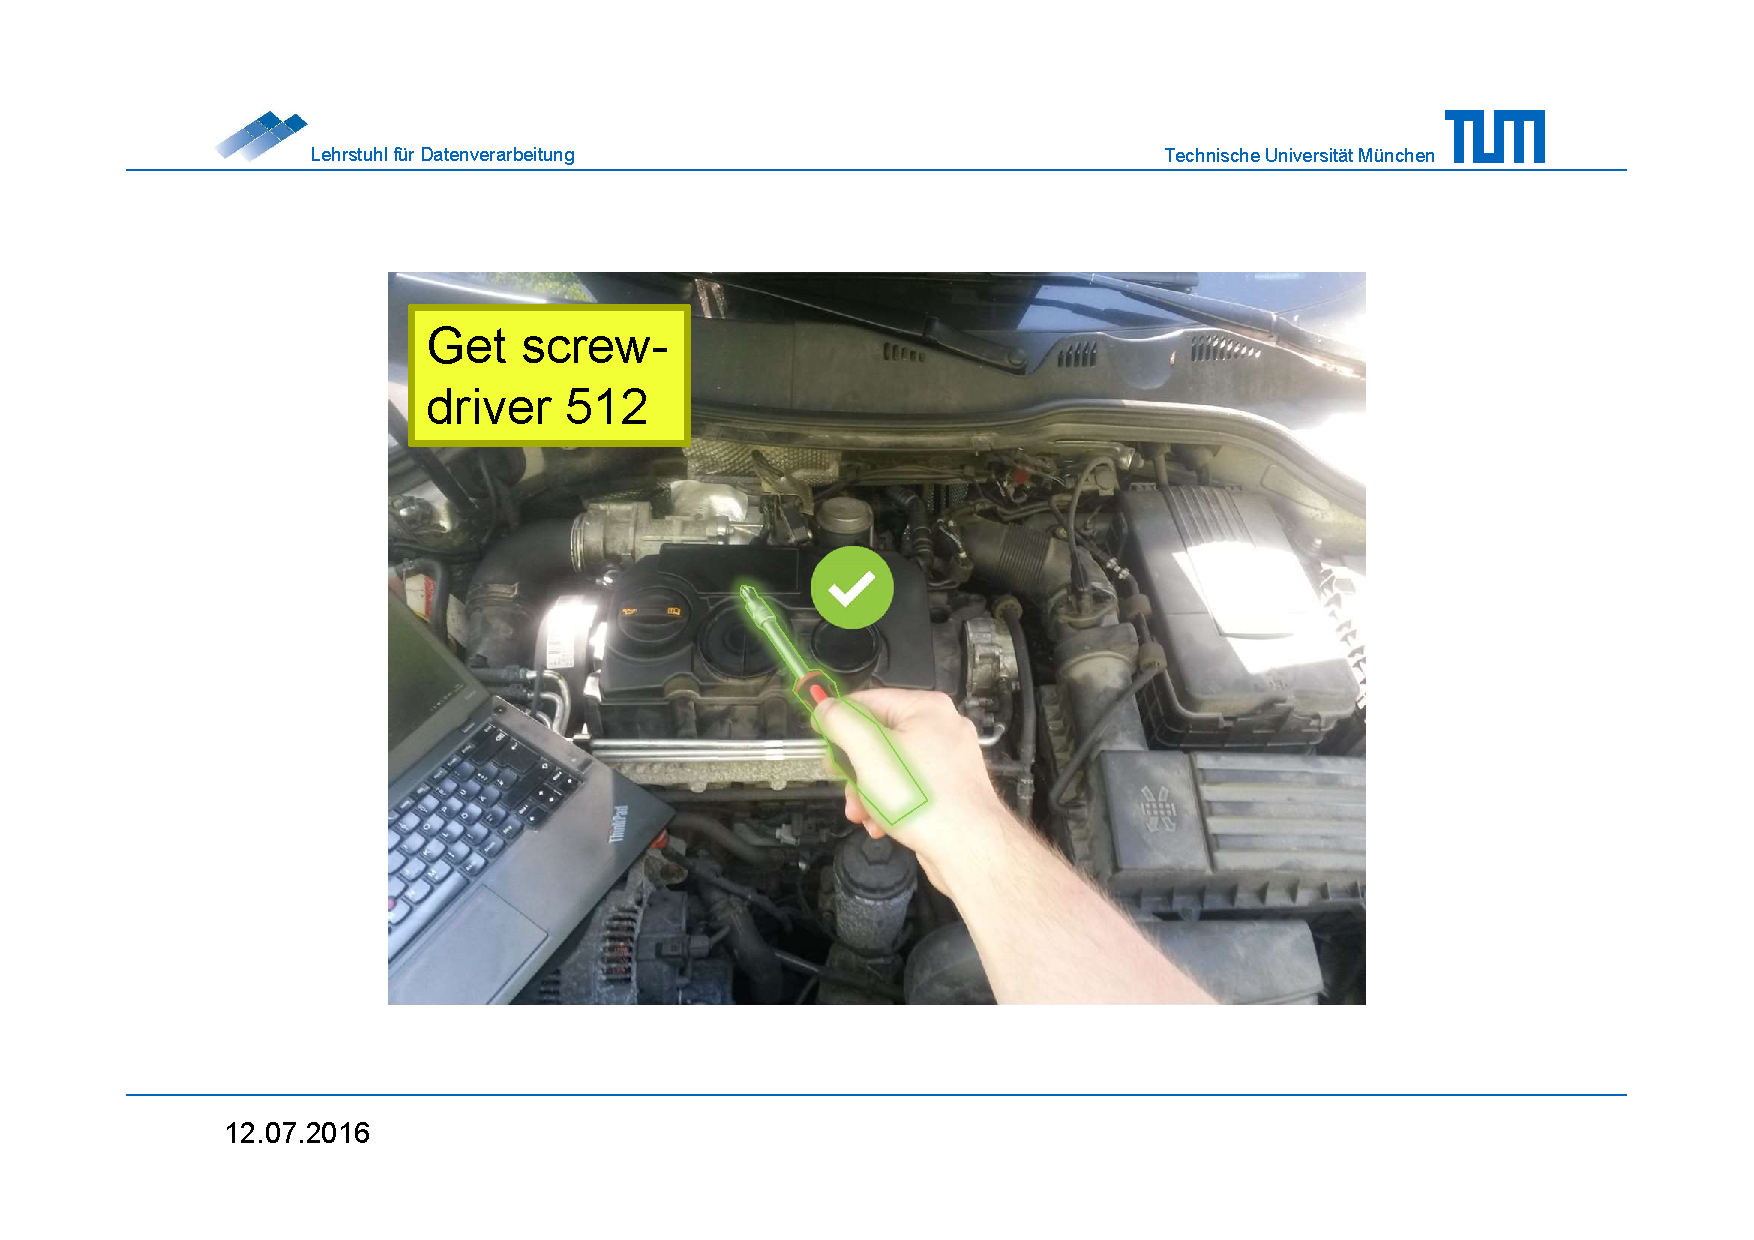
\includegraphics[width=\textwidth, trim=4cm 3cm 4cm 4cm, clip]{../images/instr-screwdriver.pdf}
			\centering
			\caption{Parties involved in the uFixit environment}
			\label{fig:instr-screwdriver}
		\end{figure}
		
		\autoref{fig:instr-hammer} and \autoref{fig:instr-screwdriver} show how one instruction step would look like. The necessary job to finish is shown in the top left - here: "Get screwdriver 512". When the user holds up a hammer, the AR device will register that and tell him that he is holding the wrong tool. After holding up the right tool, the manual will continue to the next step automatically.
		
	
	\section{Using existing AR hardware devices}
	
		
		\begin{figure}[H]
			\centering
			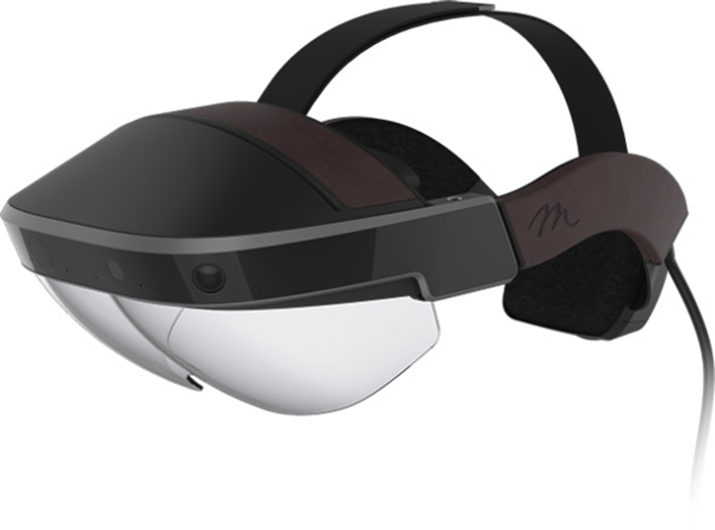
\includegraphics[width=0.5\linewidth]{../images/meta2.png}
			\caption{Meta 2 - Only one of the many devices uFixit will support}
			\label{fig:meta2}
		\end{figure}
		
		\begin{figure}[H]
			\centering
			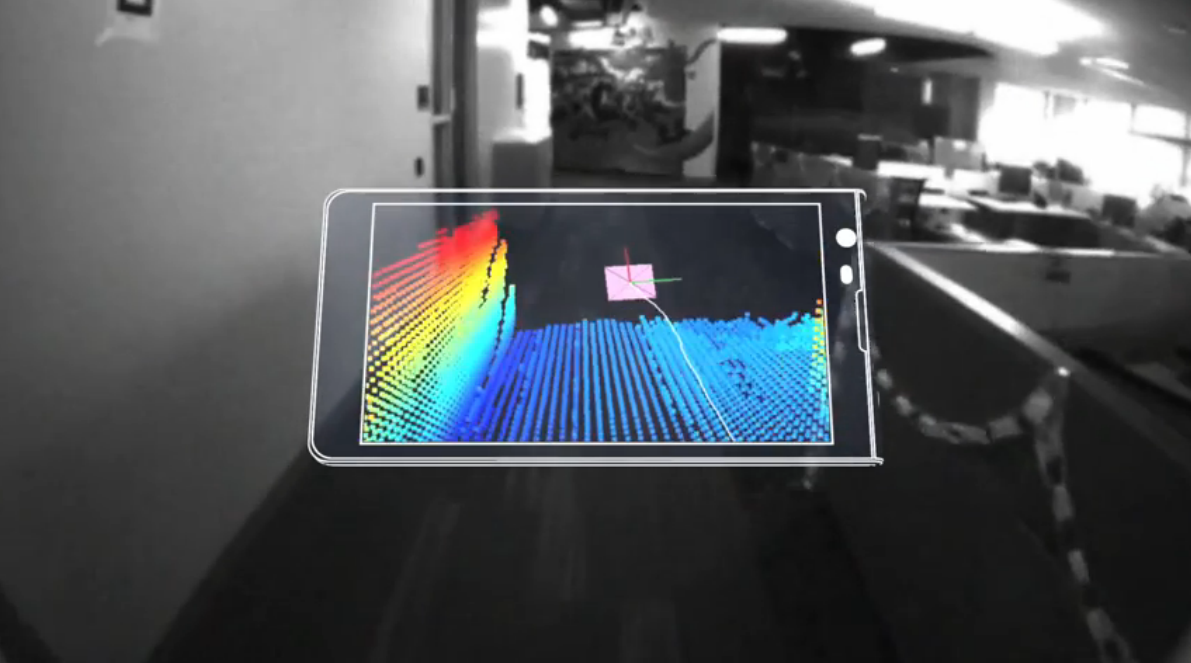
\includegraphics[width=0.7\linewidth]{../images/project-tango}
			\caption{}
			\label{fig:project-tango}
		\end{figure}
		
	

	\section{Software}
	
		- two approaches: simple CMCS, complex hard to learn 3D CAD software
		
		\subsection{Our gem: Community Manual Creation Software}
		
			- for everyone that owns an AR device
			
			- very intuitive, simple, fool proof
			
			- insert arrows by gestures, ...
	
		\subsection{3D CAD software for manufacturers}
		
			- needs good 3D model
			
			- can contain animations or see through content

			- complicated, only possible with previous training

		\subsection{Use tutorials on the device you like}
		
			- basically bring manual to as many devices as possible
			
			- classical screen
			
			- smartphones, tables with back camera
			
			- AR head mounted devices

	

%
%
%\begin{itemize}
%	\itemsep0em
%	\item consumer and helper use AR device > simple and intuitive input \begin{itemize}
%		\itemsep0em
%		\item uses AR device input! > can be different for each device!
%		\item must at all cost be intuitive! > limitations
%	\end{itemize}
%	\item manufacture has possibility for high quality software \begin{itemize}
%		\itemsep0em
%		\item 3D CAD models, ...
%		\item highly customizable
%		\item animated, ...
%	\end{itemize}
%	\item Possible interactions: \begin{itemize}
%		\itemsep0em
%		\item manuals from manufacturer to consumer
%		\item live support from manufacture to consumer
%		\item feedback from consumer to manufacture
%		\item manuals from helpers (Fixers) to consumer
%		\item live support from helpers (Fixers) to consumer
%		\item reward system (?), freelancer contracts from manufacture to helpers (Fixers)
%	\end{itemize}
%\end{itemize}
